\documentclass[10pt]{article}
\usepackage[utf8]{inputenc}
\usepackage[T1]{fontenc}
\usepackage{mathptmx}
\renewcommand{\ttdefault}{pcr}
\setlength{\emergencystretch}{3em}
\usepackage[spanish,es-nodecimaldot,es-noshorthands,es-tabla]{babel}
\usepackage[margin=1.8cm]{geometry}
\usepackage{graphicx,booktabs,xcolor,url,array,tikz,caption,float}
\usetikzlibrary{arrows.meta,positioning}
\newcommand{\pend}[1]{\textcolor{red}{[#1]}}
\renewcommand{\thetable}{S\arabic{table}}
\renewcommand{\thefigure}{S\arabic{figure}}
\captionsetup{font=small}
\title{Material suplementario\\[2pt]\large Mejorar sobre oclusión sintética no basta: aumento de oclusión y oclusión real en la detección de personas}
\author{Apaza Hilasaca, Condori Quispe, Ramos Quispe (UPeU, Juliaca)}
\date{20 de octubre de 2026; revisado el 28 de octubre de 2026}
\begin{document}
\maketitle
\noindent Todas las tablas de este suplemento las genera \texttt{shortpaper5/suplemento\_tablas.py} a partir de los ficheros de resultados del proyecto (\texttt{informes/analisis\_final/}); ninguna cifra se escribe a mano. Los análisis marcados como posteriores se declararon después de ver los resultados y no deciden ninguna hipótesis.

\section{Objetivos, método y evidencia}
\begin{table}[H]\centering\small
\caption{Correspondencia entre objetivos específicos, método, evidencia y pendientes.}
\begin{tabular}{@{}p{3.3cm}p{4.6cm}p{5.4cm}p{2.6cm}@{}}\toprule
\textbf{Objetivo} & \textbf{Método} & \textbf{Evidencia} & \textbf{Pendiente} \\\midrule
OE1. Degradación con la oclusión & AP@0.5 estratificado con regiones \emph{ignore}, tres fuentes & Modelos base entrenados en ExDark con exposición igual (10 bloques), de sin oclusión a ocluidas: ExDark 0,78--0,85 a 0,20--0,31 (severa); NightOwls 0,61--0,69 a 0,15--0,21; CityPersons 0,47--0,65 a 0,08--0,15 (\emph{heavy}) & --- \\
OE2. Efecto del aumento según el oclusor y la dosis & V3 frente a V1, control y 3 fuentes reales; parches, siluetas, difusión, geometría real y profundidad; tres dosis (H18e) & 20 de 20 controles; modelo mixto (dosis habitual, exposición igual, 12 bloques): NightOwls +0,57, CityPersons +1,06, ExDark $-1{,}11$, todos los límites superiores por debajo de +2; la dosis alta transfiere en dos fuentes (H18e-alta), pero igual en las personas sin oclusión & Curva de dosis con otros detectores; oclusión tomada de imágenes reales \\
OE3. Dependencia del detector & YOLOv11s, YOLOv11m, YOLO26s, RT-DETR-l, RetinaNet, Faster R-CNN & Mismo patrón en los cinco primeros; Faster R-CNN con siluetas pasa en NightOwls y CityPersons (H15), pero no se replica con 5 semillas (H18a, 1 de 3) ni con difusión o profundidad (H16a, H16b); RetinaNet no transfiere (H17) & Otro detector de dos etapas u otra red base \\
OE4. Dominio y volumen de datos & Re-entrenar en CityPersons (H6, H11); NightOwls de 2\,000 a 20\,000 imágenes (H7) & El déficit persiste; la ganancia dentro del dominio no se confirmó (H11) & --- \\
OE5. Mecanismo & \emph{Recall}, falsos positivos, confianza; visibilidad; realismo (H13); matriz cruzada & Los ocluidos sintéticamente siguen siendo distinguibles de los reales; menos \emph{recall} con más confianza & Prueba confirmatoria del mecanismo \\
OE6--OE7. Módulo de atención; fiabilidad de la anotación & FPS y parámetros; $\kappa$ entre anotadores & Sin ganancia del módulo (H1, H2) y FPS al 82\,\%; $\kappa$ 0,06--0,60 & Prueba en dispositivo embebido \\
\bottomrule\end{tabular}\end{table}

\noindent\textbf{Variantes del planteamiento original.} El experimento 1 tenía cuatro variantes: V1 (base), V2 (módulo de atención CBAM en el cuello), V3 (aumento de oclusión) y V4 (ambos). H1 (V4 mejora a V1) y H2 (V3 mejora más que V2) no se confirmaron, y H5 (las siluetas reducen la brecha) solo en parte, porque la brecha se cerró por empeorar lo real. El módulo de atención redujo los FPS al 82\,\% (161--184 frente a 144--157) sin ganancia en oclusión real. Desde la iteración 2 la pregunta es la transferencia y solo se comparan V1 y V3.

\section{Hipótesis y prerregistro}
La huella SHA-256 global del protocolo prueba que ningún fichero congelado cambió después del congelamiento, pero la fecha la registra el propio proyecto (\texttt{CAMBIOS\_PROTOCOLO.md}) y no un tercero. La columna «primera corrida» sale del registro de cada corrida y permite comprobar que el congelamiento es anterior al entrenamiento. Todas las fechas son de 2026.

\begin{table}[H]\centering\scriptsize
\caption{Hipótesis, predicción, congelamiento y veredicto. La huella es la del protocolo congelado (SHA-256 global, primeros 8 caracteres); la fecha es la registrada por el propio proyecto, no por un tercero. Primera corrida: inicio de la primera corrida válida del bloque, según su registro (hora local, UTC$-$5, en la laptop; UTC en RunPod: H11, H12 y H14--H17).}\label{tab:s-hip}
\resizebox{\textwidth}{!}{\begin{tabular}{@{}l p{6.3cm} l l l l p{3.2cm}@{}}\toprule
Hip. & Predicción & Archivo & Versión y huella & Congelado & Primera corrida & Veredicto \\
\midrule
H1--H3 & V4 y V3 mejoran $\geq$2 pp a V1 en oclusión (H1, H2) y la mejora se transfiere a la real (H3) & \texttt{PROTOCOLO.md} & v1.0 \texttt{c5002ea5} & 2026-09-11 08:09 & 2026-09-11 08:47 & No confirmada (0 de 3 fuentes en H3) \\
H4, H5 & Con siluetas la ganancia se transfiere (H4); menor ganancia sintética y menor brecha (H5) & \texttt{PROTOCOLO\_v2.md} & v2.0 \texttt{9915d90f} & 2026-09-12 12:51 & 2026-09-12 12:54 & H4 no confirmada (0 de 3); H5 parcial \\
H6 & Sin transferencia al re-entrenar en CityPersons & \texttt{PREREGISTRO\_H6\_H7.md} & v3.0 \texttt{e971ab8b} & 2026-09-19 16:48 & 2026-09-19 16:48 & No detectada (0 de 3) \\
H7 & Sin transferencia con 20\,000 imágenes nocturnas & \texttt{PREREGISTRO\_H6\_H7.md} & v3.1 \texttt{b0043c89} & 2026-09-25 20:58 & 2026-09-25 20:59 & No detectada (sin control) \\
H8 & Sin transferencia con RT-DETR-l & \texttt{PREREGISTRO\_H8.md} & v3.2 \texttt{51c0a2d8} & 2026-09-26 18:52 & 2026-09-26 18:52 & No detectada (0 de 3) \\
H9 & Sin transferencia con oclusores por difusión & \texttt{PREREGISTRO\_H9.md} & v3.3b \texttt{243acffb} & 2026-10-03 01:29 & 2026-10-03 01:29 & No detectada (1 de 3) \\
H9b & Ídem con 30 épocas fijas & \texttt{PREREGISTRO\_H9b.md} & v3.4 \texttt{51786d9d} & 2026-10-06 09:01 & 2026-10-06 09:02 & No detectada (0 de 3) \\
H10 & Sin transferencia con la geometría de la oclusión real & \texttt{PREREGISTRO\_H10.md} & v3.5 \texttt{1489961a} & 2026-10-06 18:27 & 2026-10-07 05:03 & No detectada (1 de 3) \\
H11 & Ganancia $\geq$2 pp en visibilidad 0,20--0,50 de CityPersons con exposición igual & \texttt{PREREGISTRO\_H11.md} & v3.6b \texttt{bd2666fd} & 2026-10-13 14:38 & 2026-10-13 20:37 & No se confirma \\
H12 & Sin transferencia con YOLOv11m (siluetas, H12a; difusión, H12b) & \texttt{PREREGISTRO\_H12.md} & v3.7b \texttt{ef6138c1} & 2026-10-13 21:06 & 2026-10-17 14:50 & No detectada (0 de 3 y 0 de 3) \\
H13 & AUC(parches) $>$ AUC(siluetas) $>$ AUC(difusión) con DINOv2 & \texttt{PREREGISTRO\_H13.md} & v3.8 \texttt{7ce00c9c} & 2026-10-17 09:48 & sin entrenamiento & Se confirma en parte \\
H14 & Sin transferencia con orden de profundidad & \texttt{PREREGISTRO\_H14.md} & v3.9 \texttt{264ac449} & 2026-10-17 10:10 & 2026-10-17 16:33 & No detectada (1 de 3) \\
H15 & Sin transferencia con Faster R-CNN & \texttt{PREREGISTRO\_H15.md} & v3.10 \texttt{b7843b3a} & 2026-10-20 16:20 & 2026-10-21 13:31 & Pasa la regla (2 de 3) \\
H16a, H16b & Con Faster R-CNN se transfiere también con difusión (H16a) y con orden de profundidad (H16b) & \texttt{PREREGISTRO\_H16\_H17.md} & v3.11 \texttt{e9b85aee} & 2026-10-22 07:50 & 2026-10-22 13:57 & Refutadas (0 de 3 y 0 de 3) \\
H17 & Sin transferencia con RetinaNet (una etapa, misma red base que H15, con su receta de referencia) & \texttt{PREREGISTRO\_H16\_H17.md} & v3.11 \texttt{e9b85aee} & 2026-10-22 07:50 & 2026-10-22 13:08 & No detectada (0 de 3) \\
\bottomrule\end{tabular}}\end{table}


\section{Registro de corridas y recetas}
Las corridas válidas son: 14 del experimento 1 (12 de V1--V4 y dos controles, sin aumento de oclusión y sin preentrenamiento), 12 de la iteración 2 (V1--V4), 6 de YOLO26s, 6 de H6, 12 de H7 (dos por peldaño de 2\,000, 5\,000 y 10\,000 con la semilla 0, y seis en 20\,000), 6 de H8 y 3 de H9 (su V1 es la de la iteración 2): 59 en los siete primeros bloques; después, 6 de H9b, 6 de H10 (su V1 es la de H9b), 6 de H11, 9 de H12, 6 de la extensión de semillas, 6 de H14, 6 de H15, 6 de H16 (V3 con difusión y con profundidad; su V1 es la de H15), 6 de H17 y 1 réplica de la V1 semilla 0 de H15 en otra máquina: 117 en total. Versiones: Ultralytics 8.4.143; PyTorch 2.11 con CUDA 12.8 en la laptop y 2.8 con CUDA 12.8 en RunPod; torchvision 0.23 para Faster R-CNN y RetinaNet. La réplica de V1 difiere de la original en $-0{,}87$ (NightOwls), $-1{,}92$ (CityPersons) y $+3{,}42$ pp (ExDark, 101 instancias), por encima del umbral de 2 pp declarado en el prerregistro: limita la comparación de H16, cuyas V1 son las de H15, entrenadas en otra máquina (en los demás bloques V1 y V3 comparten máquina, incluido H12, entrenado en un solo pod).

\begin{table}[H]\centering\scriptsize
\caption{Registro de corridas por bloque (el detalle por corrida está en \texttt{informes/analisis\_final/registro\_corridas.csv}). Épocas: entrenadas y de los pesos evaluados, mín.--máx. Con selección por validación, la época evaluada es la de máxima mAP50-95 en validación (ExDark val y val ocluida).}\label{tab:s-registro}
\resizebox{\textwidth}{!}{\begin{tabular}{@{}l l r l l l l r@{}}\toprule
Bloque & Detector & Corridas & Ép. V1 (eval./entr.) & Ép. V3 (eval./entr.) & Regla de exposición & Máquina & Horas \\
\midrule
Exp. 1 (parches) & YOLOv11s, YOLOv11s+CBAM & 14 & 2 / 22--40 & 2 / 22 & selección por validación & RTX 5050 Laptop & 7{,}8 \\
Iteración 2 (siluetas) & YOLOv11s, YOLOv11s+CBAM & 12 & 1--2 / 21--22 & 37--89 / 57--100 & selección por validación & RTX 5050 Laptop & 10{,}0 \\
Réplica YOLO26s & YOLO26s & 6 & 1--3 / 21--23 & 82--87 / 100 & selección por validación & RTX 5050 Laptop & 8{,}2 \\
H6 (CityPersons) & YOLOv11s & 6 & 38--51 / 58--71 & 85--88 / 100 & selección por validación & RTX 5050 Laptop & 18{,}4 \\
H7 peldaño 2 000 & YOLOv11s & 2 & 2 / 22 & 43 / 63 & presentaciones fijas, paciencia 1/5 & RTX 5050 Laptop & 2{,}5 \\
H7 peldaño 5 000 & YOLOv11s & 2 & 1 / 9 & 35 / 40 & presentaciones fijas, paciencia 1/5 & RTX 5050 Laptop & 3{,}5 \\
H7 peldaño 10 000 & YOLOv11s & 2 & 2 / 6 & 20 / 20 & presentaciones fijas, paciencia 1/5 & RTX 5050 Laptop & 3{,}7 \\
H7 peldaño 20 000 & YOLOv11s & 6 & 1--2 / 3--4 & 2--9 / 4--10 & presentaciones fijas, paciencia 1/5 & RTX 5050 Laptop & 9{,}0 \\
H8 (RT-DETR-l) & RT-DETR-l & 6 & --- & --- & selección por validación & RTX 5050 Laptop & 15{,}0 \\
H9 (generativa) & YOLOv11s & 3 & --- & 1--2 / 21--22 & selección por validación & RTX 5050 Laptop & 1{,}2 \\
H9b (generativa, 30 ep.) & YOLOv11s & 6 & 30 / 30 & 30 / 30 & 30 épocas fijas & RTX 5050 Laptop & 3{,}5 \\
H10 (geometría, 30 ep.) & YOLOv11s & 3 & --- & 30 / 30 & 30 épocas fijas & RTX 5050 Laptop & 1{,}9 \\
H10-s (siluetas, 30 ep.) & YOLOv11s & 3 & --- & 30 / 30 & 30 épocas fijas & RTX 5050 Laptop & 1{,}8 \\
H11 (CityPersons, 60 ep.) & YOLOv11s & 6 & 60 / 60 & 60 / 60 & 60 épocas fijas & RTX 4090 & 1{,}9 \\
H12 (YOLOv11m) & YOLOv11m & 9 & 30 / 30 & 30 / 30 & 30 épocas fijas & RTX 4090 & 1{,}0 \\
Extensión de semillas & YOLOv11s & 6 & 30 / 30 & 30 / 30 & 30 épocas fijas & RTX 4090 & 0{,}5 \\
H14 (profundidad, 30 ep.) & YOLOv11s & 6 & 30 / 30 & 30 / 30 & 30 épocas fijas & RTX 4090 & 0{,}5 \\
H15 (Faster R-CNN, 30 ep.) & Faster R-CNN R50-FPN v2 & 6 & 30 / 30 & 30 / 30 & 30 épocas fijas & RTX 4090 & 2{,}6 \\
H16a (Faster R-CNN, generativa) & Faster R-CNN R50-FPN v2 & 3 & --- & 30 / 30 & 30 épocas fijas & RTX 4090 & 1{,}9 \\
H16b (Faster R-CNN, profundidad) & Faster R-CNN R50-FPN v2 & 3 & --- & 30 / 30 & 30 épocas fijas & RTX 4090 & 1{,}9 \\
H17 (RetinaNet, 30 ep.) & RetinaNet R50-FPN v2 & 6 & 30 / 30 & 30 / 30 & 30 épocas fijas & RTX 4090 & 2{,}5 \\
Réplica de V1 entre pods & Faster R-CNN R50-FPN v2 & 1 & 30 / 30 & --- & 30 épocas fijas & RTX 4090 & 0{,}2 \\
\midrule Total & & 117 & & & & & 99{,}3 \\
\bottomrule\end{tabular}}\end{table}


\begin{table}[H]\centering\small
\caption{Receta de entrenamiento por detector. El aumento base (idéntico en V1 y V3) son los valores de Ultralytics 8.4 fijados en \texttt{config/aumento\_base.yaml}: HSV (0,015; 0,7; 0,4), traslación 0,1, escala 0,5, volteo horizontal 0,5, mosaico 1,0 sin mosaico en las 10 últimas épocas.}
\begin{tabular}{@{}p{2.6cm}p{2.2cm}p{2.6cm}p{1.9cm}p{1.6cm}p{1.6cm}p{2.6cm}@{}}\toprule
Detector & Optimizador & Tasa (final) & Calentamiento & Decaimiento & Lote & Épocas \\\midrule
YOLOv11s/m, YOLO26s & SGD, momento 0,937 & 0,002 (lineal a 1\,\%) & 3 épocas & $5\cdot10^{-4}$ & 16 & hasta 100 (pac. 20) o 30/60 fijas \\
RT-DETR-l & AdamW, $\beta_1$ 0,9 & $10^{-4}$ (lineal a 1\,\%) & 3 épocas, sesgo 0 & $10^{-4}$ & 8 (acum. a 64) & hasta 100 (pac. 20) \\
Faster R-CNN R50-FPN v2 & SGD, momento 0,9 & 0,01, $\times$0,1 en 20 y 27 & 500 iteraciones & $10^{-4}$ & 8 & 30 fijas \\
RetinaNet R50-FPN v2 & SGD, momento 0,9 & 0,005, $\times$0,1 en 20 y 27 & 500 iteraciones & $10^{-4}$ & 8 & 30 fijas \\
\bottomrule\end{tabular}\end{table}

\section{Aumento y control de cada familia}
\begin{table}[H]\centering\small
\caption{Parámetros del aumento (entrenamiento) y del control (prueba). El control usa las imágenes de prueba del dominio de entrenamiento y todas sus personas válidas (las 841 de ExDark test; CityPersons val en H6 y H11, \texttt{cp\_silueta\_severa}), con cobertura de 0,70 a 1,00 y oclusores que el modelo no vio al entrenar.}
\begin{tabular}{@{}p{2.2cm}p{7.0cm}p{6.6cm}@{}}\toprule
Familia & Entrenamiento (V3) & Control \\\midrule
Parches & Rectángulos de textura (0,4), recortes de objetos (0,5) u opacos (0,1); $p=0{,}5$ por imagen, 1--3 personas, cobertura 0,30--0,85; banco de recortes de \emph{train} & \texttt{opaco\_severa}: banda de borde opaca; banco de recortes de \emph{test}, disjunto del de \emph{train} \\
Siluetas & Siluetas con máscara de objetos y personas reales (persona con prob. 0,5), ajuste de luminancia; mismos $p$, número y cobertura; banco \texttt{siluetas\_train} & \texttt{silueta\_severa}: banco \texttt{siluetas\_test} (imágenes disjuntas) \\
Difusión & Stable Diffusion 1.5 \emph{inpainting}, 20 pasos, guía 7,5, diez objetos de COCO («a parked car», «a bicycle»…) con el sufijo «at night, low light, realistic photo»; dos versiones por imagen generadas de antemano y sustituidas con $p=0{,}15$ (con mosaico) o 0,5 (sin él); control de calidad con YOLOv11s-seg (se rechaza si $>$30\,\% de la máscara sigue siendo persona) & \texttt{generativa\_severa}: mismas indicaciones y modelo, generadas de nuevo sobre las imágenes de prueba con otras semillas (96,2\,\% aceptadas) \\
Geometría real & Siluetas colocadas sobre la región oculta de patrones de visibilidad reales de CityPersons \emph{train}, cobertura 0,40--0,95 & \texttt{geometria\_severa}: patrones de la validación interna y banco de \emph{test} (IoU medio recorte--región oculta 0,61) \\
Profundidad & Recortes de objetos apoyados en el suelo delante de la persona y compuestos solo donde la escena está más lejos (Depth Anything V2 Small); 2 versiones por imagen, misma sustitución que difusión & \texttt{profundidad\_severa}: banco \texttt{siluetas\_test} \\
\bottomrule\end{tabular}\end{table}

\begin{figure}[H]\centering
\includegraphics[width=0.92\textwidth]{fig_cualitativa_es.png}
\caption{Arriba: oclusión real anotada en las tres fuentes (caja naranja: persona evaluada). Abajo: la misma persona de ExDark test en el control de cada familia sintética (caja verde).}
\end{figure}

\begin{figure}[H]\centering
\begin{tikzpicture}[n/.style={draw,rounded corners,align=center,font=\footnotesize,minimum height=0.9cm,text width=2.5cm},a/.style={-Stealth}]
\node[n] (d) {ExDark train\\(1\,183 imágenes)};
\node[n,right=0.5cm of d] (b) {Aumento base\\(igual en V1 y V3)};
\node[n,right=0.5cm of b] (o) {Oclusión sintética\\(solo V3; 5 familias)};
\node[n,right=0.5cm of o] (t) {Entrenamiento\\(épocas fijas o selección)};
\node[n,below=0.6cm of t] (e) {Evaluación AP@0.5\\con regiones \emph{ignore}};
\node[n,left=0.5cm of e] (c) {Control sintético\\(oclusores no vistos)};
\node[n,left=0.5cm of c] (r) {3 fuentes reales\\NO, CP, EX};
\node[n,left=0.5cm of r] (v) {IC por imágenes y jerárquico; regla 2 de 3};
\draw[a] (d)--(b); \draw[a] (b)--(o); \draw[a] (o)--(t); \draw[a] (t)--(e); \draw[a] (c)--(e); \draw[a] (r) to[bend left=20] (e); \draw[a] (e) to[bend left=25] (v);
\end{tikzpicture}
\caption{Tubería de cada bloque. La oclusión se aplica sobre la imagen RGB, después del aumento base y antes del formateo, solo en entrenamiento; la validación y la prueba nunca se ocluyen salvo en el control.}
\end{figure}

\section{Todas las celdas y análisis estadístico}
\begin{table}[H]\centering\scriptsize
\caption{Todas las celdas: V3$-$V1 en AP@0.5 (pp), IC 95\,\% por imágenes (1\,000 réplicas) y jerárquico (semillas e imágenes, 2\,000), 3 semillas por variante. * pasa: estimación $\geq+2$ e IC por imágenes $>0$. $\dagger$ descarta una ganancia de $+2$ pp (límite superior del IC por imágenes $<+2$). Exposición: igual (épocas fijas), desigual (V1 y V3 seleccionados en épocas distintas por validación) o temprana (ambas en las épocas 1--2).}\label{tab:s-celdas}
\resizebox{\textwidth}{!}{\begin{tabular}{@{}l l l r l l | l r l l@{}}\toprule
Bloque & Exp. & Celda & $\Delta$ & IC imágenes & IC jerárquico & Celda & $\Delta$ & IC imágenes & IC jerárquico \\
\midrule
H3 & temprana & Control & +60{,}92* & [+58{,}50; +63{,}41] & [+56{,}75; +64{,}95] & NO & $-$3{,}17$^\dagger$ & [$-$4{,}58; $-$1{,}74] & [$-$7{,}94; +2{,}10] \\
 & & CP & $-$0{,}36$^\dagger$ & [$-$1{,}06; +0{,}31] & [$-$2{,}42; +1{,}62] & EX & $-$3{,}25$^\dagger$ & [$-$5{,}81; $-$0{,}21] & [$-$7{,}11; +0{,}89] \\
H4 & desigual & Control & +10{,}63* & [+9{,}42; +12{,}15] & [+8{,}95; +12{,}50] & NO & $-$16{,}79$^\dagger$ & [$-$19{,}59; $-$13{,}96] & [$-$20{,}41; $-$12{,}96] \\
 & & CP & $-$3{,}94$^\dagger$ & [$-$5{,}66; $-$2{,}41] & [$-$7{,}14; $-$1{,}02] & EX & $-$5{,}02$^\dagger$ & [$-$10{,}72; +0{,}50] & [$-$11{,}89; +1{,}28] \\
H4-Y26 & desigual & Control & +12{,}01* & [+10{,}61; +13{,}57] & [+10{,}32; +13{,}79] & NO & $-$14{,}31$^\dagger$ & [$-$17{,}35; $-$11{,}10] & [$-$18{,}07; $-$10{,}14] \\
 & & CP & $-$4{,}42$^\dagger$ & [$-$5{,}95; $-$2{,}63] & [$-$6{,}89; $-$1{,}65] & EX & $-$3{,}51$^\dagger$ & [$-$8{,}38; +1{,}21] & [$-$9{,}48; +1{,}86] \\
H6 & desigual & Control & +23{,}74* & [+21{,}09; +26{,}51] & [+20{,}44; +27{,}22] & NO & $-$1{,}35$^\dagger$ & [$-$2{,}85; +0{,}20] & [$-$3{,}47; +0{,}68] \\
 & & CP & +1{,}82 & [+0{,}31; +3{,}31] & [$-$0{,}86; +4{,}42] & EX & +0{,}94 & [$-$2{,}53; +4{,}72] & [$-$4{,}06; +6{,}68] \\
H7 & desigual & NO & $-$1{,}43$^\dagger$ & [$-$3{,}98; +1{,}00] & [$-$4{,}45; +1{,}56] & CP & $-$3{,}94$^\dagger$ & [$-$5{,}62; $-$2{,}27] & [$-$8{,}15; +0{,}78] \\
 & & EX & $-$9{,}15$^\dagger$ & [$-$13{,}94; $-$5{,}66] & [$-$17{,}22; $-$3{,}26] & & & & \\
H8 & desigual & Control & +10{,}97* & [+9{,}57; +12{,}36] & [+9{,}32; +12{,}83] & NO & $-$6{,}98$^\dagger$ & [$-$8{,}95; $-$5{,}11] & [$-$11{,}16; $-$2{,}81] \\
 & & CP & $-$3{,}47$^\dagger$ & [$-$4{,}86; $-$1{,}81] & [$-$6{,}27; $-$0{,}74] & EX & $-$2{,}21$^\dagger$ & [$-$6{,}16; +1{,}59] & [$-$7{,}61; +3{,}39] \\
H9 & temprana & Control & +2{,}60* & [+2{,}12; +3{,}09] & [+0{,}25; +4{,}33] & NO & $-$1{,}93$^\dagger$ & [$-$2{,}89; $-$0{,}88] & [$-$3{,}87; $-$0{,}12] \\
 & & CP & +1{,}23 & [+0{,}36; +2{,}11] & [$-$1{,}70; +4{,}03] & EX & +2{,}82* & [+0{,}37; +5{,}99] & [$-$1{,}23; +7{,}40] \\
H9b & igual & Control & +15{,}23* & [+14{,}00; +17{,}16] & [+13{,}81; +17{,}45] & NO & +0{,}01$^\dagger$ & [$-$1{,}02; +1{,}20] & [$-$1{,}60; +1{,}82] \\
 & & CP & +1{,}52 & [+0{,}79; +2{,}66] & [$-$0{,}02; +3{,}39] & EX & $-$3{,}03$^\dagger$ & [$-$6{,}77; +0{,}99] & [$-$8{,}85; +2{,}89] \\
H11 & igual & Control & +24{,}66* & [+21{,}62; +27{,}47] & [+21{,}44; +28{,}09] & NO & +1{,}95 & [+0{,}93; +3{,}21] & [$-$0{,}16; +4{,}66] \\
 & & CP & +1{,}31 & [$-$0{,}28; +2{,}78] & [$-$0{,}85; +3{,}46] & EX & $-$2{,}44 & [$-$6{,}77; +2{,}36] & [$-$7{,}34; +3{,}23] \\
H10 & igual & Control & +18{,}39* & [+15{,}61; +21{,}30] & [+15{,}57; +21{,}47] & NO & $-$2{,}05$^\dagger$ & [$-$3{,}26; $-$0{,}92] & [$-$4{,}62; +0{,}29] \\
 & & CP & +2{,}37* & [+1{,}52; +3{,}52] & [+0{,}63; +4{,}61] & EX & $-$4{,}88$^\dagger$ & [$-$9{,}08; $-$0{,}82] & [$-$11{,}58; +1{,}03] \\
H10-s & igual & Control & +10{,}99* & [+9{,}62; +12{,}62] & [+9{,}58; +12{,}68] & NO & $-$1{,}12$^\dagger$ & [$-$2{,}13; +0{,}08] & [$-$2{,}58; +0{,}49] \\
 & & CP & +2{,}26* & [+1{,}44; +3{,}47] & [+0{,}72; +4{,}04] & EX & $-$3{,}50$^\dagger$ & [$-$7{,}64; +0{,}08] & [$-$9{,}63; +1{,}86] \\
H12a & igual & Control & +14{,}45* & [+12{,}76; +16{,}37] & [+12{,}67; +16{,}46] & NO & $-$0{,}39$^\dagger$ & [$-$1{,}55; +0{,}89] & [$-$3{,}92; +2{,}77] \\
 & & CP & +0{,}25$^\dagger$ & [$-$0{,}63; +1{,}27] & [$-$1{,}32; +2{,}12] & EX & +3{,}04 & [$-$1{,}07; +6{,}63] & [$-$2{,}63; +8{,}31] \\
H12b & igual & Control & +19{,}04* & [+17{,}49; +21{,}03] & [+17{,}35; +21{,}21] & NO & +0{,}78 & [$-$0{,}42; +2{,}16] & [$-$3{,}21; +4{,}28] \\
 & & CP & +1{,}11 & [+0{,}14; +2{,}16] & [$-$0{,}47; +2{,}89] & EX & $-$0{,}56 & [$-$4{,}07; +3{,}19] & [$-$5{,}77; +5{,}06] \\
H14 & igual & Control & +7{,}42* & [+6{,}40; +8{,}79] & [+6{,}13; +9{,}13] & NO & $-$1{,}50$^\dagger$ & [$-$2{,}75; $-$0{,}37] & [$-$3{,}40; +0{,}26] \\
 & & CP & $-$0{,}16$^\dagger$ & [$-$1{,}21; +0{,}75] & [$-$1{,}85; +1{,}31] & EX & +5{,}49* & [+1{,}63; +9{,}30] & [$-$0{,}35; +11{,}14] \\
H15 & igual & Control & +14{,}72* & [+13{,}04; +16{,}66] & [+12{,}97; +16{,}63] & NO & +3{,}28* & [+1{,}64; +4{,}79] & [+0{,}67; +5{,}81] \\
 & & CP & +2{,}33* & [+1{,}01; +3{,}69] & [+0{,}13; +4{,}92] & EX & $-$1{,}00 & [$-$5{,}61; +3{,}24] & [$-$6{,}71; +4{,}04] \\
\bottomrule\end{tabular}}\end{table}


\begin{figure}[H]\centering
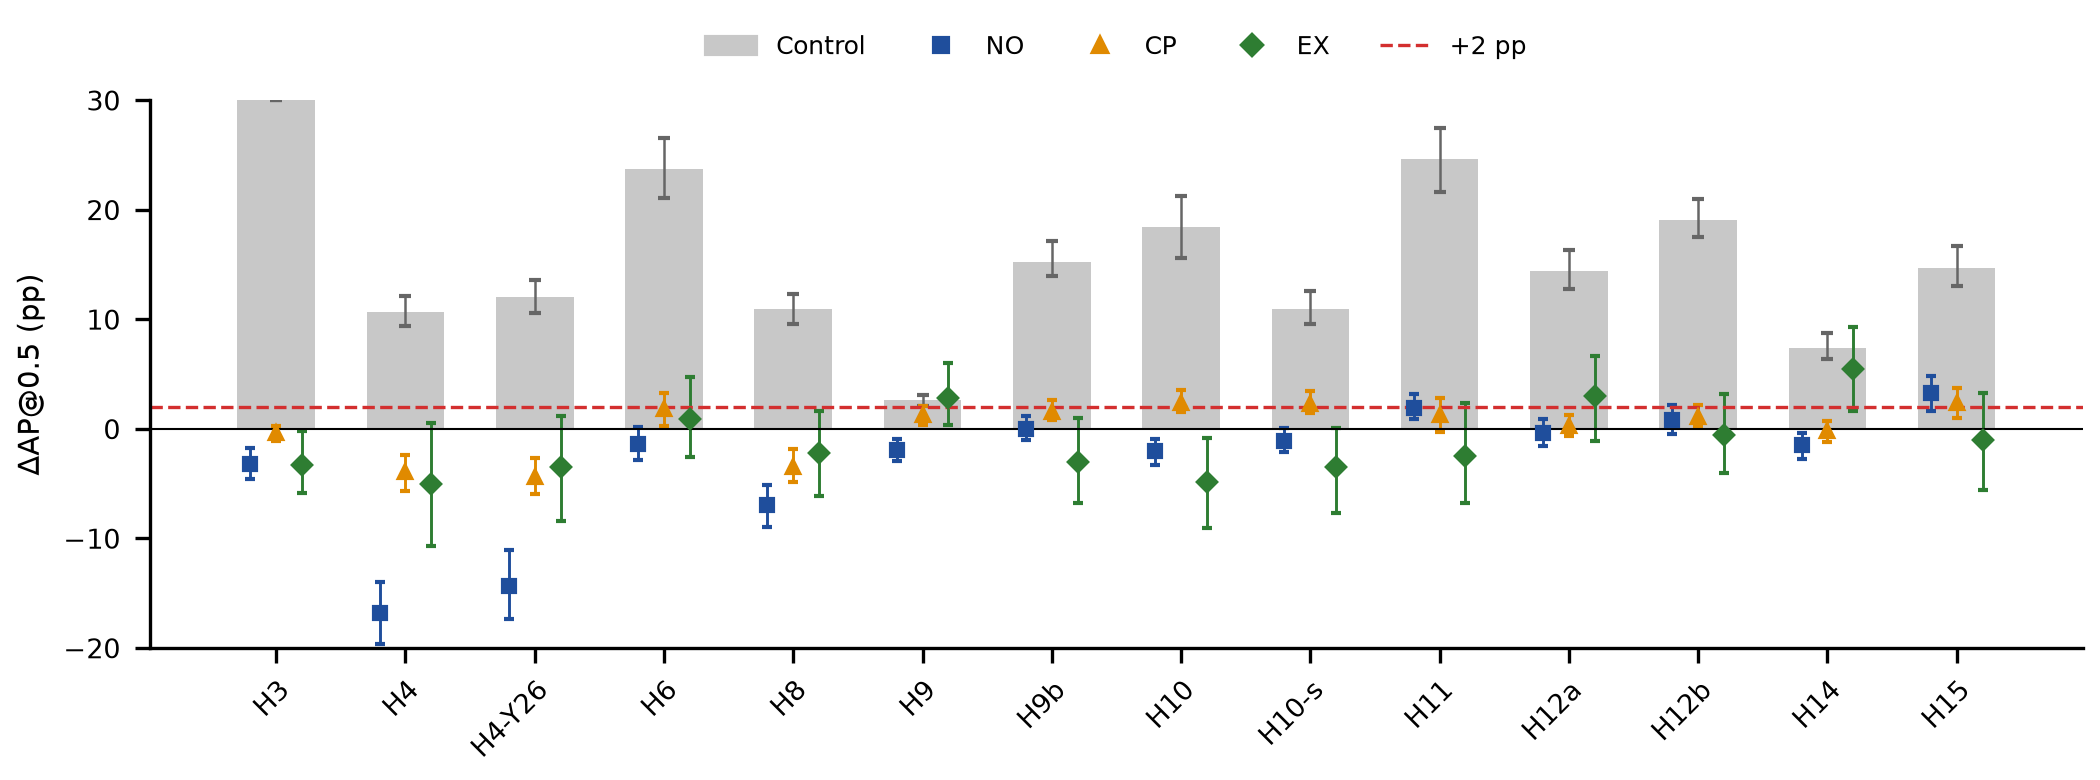
\includegraphics[width=\textwidth]{fig_gap_ic_es.png}
\caption{Control sintético (barras) y fuentes reales (marcadores) por bloque, con IC del 95\,\% por imágenes. La barra de H3 se corta en +30 (+60,9).}
\end{figure}

\begin{table}[H]\centering\scriptsize
\caption{Recuentos y análisis estadísticos declarados (posteriores): 13 bloques con control, 39 celdas reales. Modelo mixto: ganancia real $\sim$ ganancia sintética (estandarizada) + fuente, con intercepto aleatorio por bloque.}\label{tab:s-estad}
\begin{tabular}{@{}p{5.0cm} p{2.9cm}@{}}\toprule
Celdas reales que pasan (estimación $\geq+2$ e IC $>0$) & 4 de 39 (con IC jerárquico: 2) \\
Descartan una ganancia de +2 pp (no superioridad, unilateral 2,5 \%) & 24 de 39 (jerárquico: 19) \\
Exposición igual (21 celdas): pasan / negativas con IC / media & 3 / 3 / +0{,}02 pp \\
Exposición desigual (12 celdas): pasan / negativas con IC / media & 0 / 6 / $-$4{,}94 pp \\
Selección temprana en ambas (6 celdas): pasan / negativas con IC / media & 1 / 3 / $-$0{,}78 pp \\
Sin el indicador de ExDark: celdas que pasan; bloques con 2 de 2 & 2 de 26; 0 \\
DE entre semillas del AP@0.5 de V1 en fuentes reales (mediana; máx.) & 1{,}53; 4{,}10 pp (26 grupos) \\
$\rho$ de Spearman, NO (IC bootstrap de bloques) & +0{,}41 [$-$0{,}18; +0{,}85] \\
$\rho$ de Spearman, CP (IC bootstrap de bloques) & +0{,}30 [$-$0{,}26; +0{,}71] \\
$\rho$ de Spearman, EX (IC bootstrap de bloques) & $-$0{,}15 [$-$0{,}67; +0{,}54] \\
Modelo mixto: pendiente por DE de ganancia sintética (14{,}0 pp) & +0{,}11 pp [$-$1{,}74; +1{,}95], $p=0{,}91$ \\
Ídem sin H3 & +0{,}66 pp [$-$1{,}31; +2{,}64], $p=0{,}51$ \\
\bottomrule\end{tabular}\end{table}


\noindent\textbf{Por qué +2 pp (revisión del 22/10).} Además de superar la desviación típica entre semillas del AP de V1 (mediana 1,5 pp), +2 pp es relevante en la práctica: sobre el AP@0.5 mediano de V1 en las personas ocluidas (0,17 en NightOwls, 0,15 en CityPersons \emph{heavy} y 0,26 en el indicador de ExDark) equivale a una mejora relativa del 12\,\%, 13\,\% y 8\,\%. Y es detectable: el error típico mediano de una diferencia V3$-$V1 es 0,78 pp (0,68 en NightOwls, 0,52 en CityPersons y 1,98 en ExDark), así que, salvo en el indicador de ExDark, un efecto de +2 pp queda a más de 2,5 errores típicos del cero.

\section{Matriz cruzada de controles}
Si el control solo midiera la memoria del oclusor concreto, un modelo ganaría en su propio control y no en el de las demás familias. La tabla~\ref{tab:s-cruzada} evalúa cada familia en el control de todas. Pasan 13 de las 20 celdas fuera de la diagonal (también 13 con el IC jerárquico): el aumento se transfiere de una oclusión sintética a otra, pero no a la real (recuento primario: 5 de 33). Los parches del experimento 1 y la difusión se quedan casi en su propio control.

\begin{table}[H]\centering\scriptsize
\caption{Matriz cruzada de controles: V3$-$V1 (AP@0.5, pp, 3 semillas) de cada familia de entrenamiento (filas) en el control severo de cada familia (columnas), IC por imágenes entre corchetes. Todos los controles usan imágenes de ExDark test e instancias de oclusor no vistas en el entrenamiento. Parches: modelos del experimento 1 (épocas 1--2); el resto, 30 épocas fijas.}\label{tab:s-cruzada}
\setlength{\tabcolsep}{2pt}\begin{tabular}{@{}l ccccc@{}}\toprule
Entrenado con & Parches & Siluetas & Generativa & Geometría real & Profundidad \\ \midrule
Parches & \textbf{+60{,}9} & +1{,}3 & +3{,}0 & +0{,}9 & +0{,}8 \\
 & {\tiny [+58{,}52; +63{,}35]} & {\tiny [+0{,}79; +1{,}86]} & {\tiny [+2{,}54; +3{,}71]} & {\tiny [+0{,}15; +1{,}75]} & {\tiny [+0{,}49; +1{,}21]} \\[2pt]
Siluetas & +18{,}1 & \textbf{+11{,}0} & +2{,}3 & +15{,}8 & +4{,}3 \\
 & {\tiny [+16{,}56; +19{,}99]} & {\tiny [+9{,}63; +12{,}57]} & {\tiny [+1{,}84; +3{,}14]} & {\tiny [+13{,}48; +18{,}61]} & {\tiny [+3{,}55; +5{,}07]} \\[2pt]
Generativa & +7{,}6 & +0{,}4 & \textbf{+15{,}2} & +1{,}9 & +0{,}7 \\
 & {\tiny [+6{,}71; +8{,}63]} & {\tiny [+0{,}02; +0{,}87]} & {\tiny [+14{,}01; +17{,}20]} & {\tiny [+0{,}97; +2{,}97]} & {\tiny [+0{,}31; +1{,}05]} \\[2pt]
Geometría real & +13{,}7 & +6{,}3 & +1{,}7 & \textbf{+18{,}4} & +2{,}2 \\
 & {\tiny [+12{,}37; +15{,}26]} & {\tiny [+5{,}19; +7{,}48]} & {\tiny [+1{,}28; +2{,}55]} & {\tiny [+15{,}77; +21{,}26]} & {\tiny [+1{,}64; +2{,}79]} \\[2pt]
Profundidad & +8{,}3 & +6{,}7 & +3{,}1 & +11{,}7 & \textbf{+7{,}4} \\
 & {\tiny [+7{,}32; +9{,}60]} & {\tiny [+5{,}66; +7{,}95]} & {\tiny [+2{,}40; +3{,}72]} & {\tiny [+9{,}67; +14{,}52]} & {\tiny [+6{,}35; +8{,}79]} \\[2pt]
\bottomrule\end{tabular}\end{table}


\section{Análisis secundarios}
\begin{table}[H]\centering\scriptsize
\caption{Análisis secundarios declarados: cinco semillas (YOLOv11s, 30 épocas), escalera de NightOwls de H7 (semilla 0, NightOwls ocluida) y tasa de fallos MR$^{-2}$ (pp; negativo = el aumento pierde menos personas).}\label{tab:s-extra}
\setlength{\tabcolsep}{2.5pt}\begin{tabular}{@{}l l r l@{}}\toprule
Análisis & Celda & $\Delta$ & IC (imágenes / jerárquico) \\
\midrule
H9b, 5 semillas & NO & $-$0{,}45 & [$-$1{,}28; +0{,}60] / [$-$1{,}99; +1{,}23] \\
H9b, 5 semillas & CP & +0{,}22 & [$-$0{,}37; +1{,}02] / [$-$1{,}39; +2{,}00] \\
H9b, 5 semillas & EX & $-$1{,}75 & [$-$4{,}79; +1{,}83] / [$-$6{,}80; +3{,}46] \\
H10-s, 5 semillas & NO & $-$1{,}06 & [$-$1{,}89; $-$0{,}03] / [$-$2{,}36; +0{,}39] \\
H10-s, 5 semillas & CP & +2{,}06 & [+1{,}40; +2{,}99] / [+0{,}26; +4{,}17] \\
H10-s, 5 semillas & EX & $-$2{,}06 & [$-$5{,}37; +0{,}97] / [$-$7{,}27; +2{,}65] \\
\midrule
H7, 2000 img. & NO & +0{,}66 & [$-$3{,}31; +5{,}13] \\
H7, 5000 img. & NO & $-$1{,}12 & [$-$4{,}99; +3{,}10] \\
H7, 10000 img. & NO & +4{,}38 & [+0{,}17; +8{,}06] \\
H7, 20000 img. & NO & $-$1{,}43 & [$-$3{,}98; +1{,}00] \\
\midrule
MR$^{-2}$ H3 & \multicolumn{3}{l}{NO +2{,}9; CP $-$0{,}0; EX +2{,}4} \\
MR$^{-2}$ H4 & \multicolumn{3}{l}{NO +13{,}4; CP +1{,}6; EX +8{,}2} \\
MR$^{-2}$ H4-Y26 & \multicolumn{3}{l}{NO +10{,}3; CP +1{,}6; EX +3{,}4} \\
MR$^{-2}$ H6 & \multicolumn{3}{l}{NO +2{,}1; CP $-$3{,}2; EX +0{,}2 (1 mejora $\geq$2 con IC)} \\
MR$^{-2}$ H7 & \multicolumn{3}{l}{NO +1{,}4; CP +2{,}4; EX +14{,}7} \\
MR$^{-2}$ H8 & \multicolumn{3}{l}{NO +6{,}3; CP +2{,}1; EX +2{,}8} \\
MR$^{-2}$ H9 & \multicolumn{3}{l}{NO +1{,}4; CP $-$0{,}9; EX $-$3{,}2 (1 mejora $\geq$2 con IC)} \\
MR$^{-2}$ H9b & \multicolumn{3}{l}{NO $-$0{,}2; CP $-$1{,}2; EX +2{,}9} \\
MR$^{-2}$ H10 & \multicolumn{3}{l}{NO +1{,}7; CP $-$1{,}5; EX +4{,}1} \\
MR$^{-2}$ H10-s & \multicolumn{3}{l}{NO +0{,}8; CP $-$1{,}5; EX +3{,}0} \\
MR$^{-2}$ H11 & \multicolumn{3}{l}{NO $-$1{,}8; CP $-$0{,}6; EX +1{,}1} \\
MR$^{-2}$ H12a & \multicolumn{3}{l}{NO +0{,}5; CP +0{,}0; EX $-$4{,}0 (1 mejora $\geq$2 con IC)} \\
MR$^{-2}$ H12b & \multicolumn{3}{l}{NO +0{,}3; CP $-$0{,}5; EX +0{,}6} \\
MR$^{-2}$ H14 & \multicolumn{3}{l}{NO +0{,}9; CP +0{,}5; EX $-$3{,}4 (1 mejora $\geq$2 con IC)} \\
MR$^{-2}$ H15 & \multicolumn{3}{l}{NO $-$2{,}0; CP $-$1{,}4; EX $-$1{,}3} \\
MR$^{-2}$ H16a & \multicolumn{3}{l}{NO +0{,}1; CP +0{,}0; EX +0{,}3} \\
MR$^{-2}$ H16b & \multicolumn{3}{l}{NO $-$0{,}1; CP $-$0{,}5; EX +0{,}8} \\
MR$^{-2}$ H17 & \multicolumn{3}{l}{NO +2{,}3; CP +0{,}2; EX +4{,}4} \\
\bottomrule\end{tabular}\end{table}


\begin{table}[H]\centering\scriptsize
\caption{CityPersons por visibilidad anotada (análisis posterior declarado): V3$-$V1 en AP@0.5 (pp) por tramo; las demás personas son regiones \emph{ignore}.}\label{tab:s-vis}
\setlength{\tabcolsep}{2.5pt}\begin{tabular}{@{}l rrrrrr@{}}\toprule
Bloque & 0{,}20--0{,}35 & 0{,}35--0{,}50 & 0{,}50--0{,}65 & 0{,}65--0{,}80 & 0{,}80--0{,}90 & 0{,}90--1{,}00 \\ \midrule
H3 & $-$0{,}1 & +0{,}4 & +0{,}3 & +1{,}2 & +1{,}1 & +1{,}7 \\
H4 & $-$0{,}1 & $-$1{,}8 & $-$5{,}4 & $-$9{,}7 & $-$13{,}8 & $-$11{,}9 \\
H4-Y26 & $-$0{,}3 & $-$1{,}9 & $-$5{,}8 & $-$8{,}5 & $-$12{,}8 & $-$9{,}9 \\
H6 & +4{,}3 & +3{,}4 & +2{,}1 & +0{,}4 & +0{,}8 & +0{,}4 \\
H7 & +0{,}3 & $-$1{,}3 & $-$8{,}1 & $-$14{,}1 & $-$16{,}4 & $-$15{,}6 \\
H8 & $-$0{,}1 & $-$2{,}5 & $-$6{,}3 & $-$9{,}2 & $-$9{,}8 & $-$7{,}2 \\
H9 & +0{,}3 & +1{,}0 & +1{,}0 & +2{,}5 & +3{,}0 & +2{,}1 \\
H9b & +0{,}0 & +0{,}8 & +2{,}6 & +3{,}9 & +5{,}9 & +5{,}2 \\
\bottomrule\end{tabular}\end{table}


\noindent\textbf{Referencia con modelos de fundación.} OWLv2~(Minderer et al., NeurIPS 2023) y Grounding DINO~(Liu et al., ECCV 2024) sin ajuste no superan a los detectores de COCO en NightOwls ocluida ni en CityPersons \emph{heavy}, que entrenar en CityPersons lleva a 0,58--0,59 (\texttt{informes/reporte\_referencia\_fundacion.md}).

\noindent\textbf{Realismo (H13).} Cobertura media conseguida: parches 0,56, siluetas 0,54, geometría 0,47 y difusión 0,32 (el control de calidad dejó sin ocluir a 146 de 400 personas), frente a 0,55 de la oclusión real. No hay máscaras de oclusor reales en CityPersons (solo la caja visible y la completa), por lo que no se puede calcular el IoU entre máscaras sintéticas y reales; la familia de geometría real reproduce por construcción la región oculta de patrones reales (IoU medio 0,61 entre recorte y región oculta) y tampoco se transfiere (H10).

\noindent\textbf{KID sobre la región del oclusor (análisis posterior).} Con DINOv2 sobre la parte ocluida (real: franja de la caja completa fuera de la caja visible anotada; sintética: rectángulo de los píxeles que cambian respecto de la misma persona sin ocluir), la distancia al oclusor real es 2,56 [2,08; 3,17] con parches, 3,39 [2,63; 4,23] con siluetas, 2,75 [1,91; 3,51] con geometría y 2,50 [1,87; 3,02] con difusión (248 regiones; el control de calidad dejó 152 sin ocluir), frente a 3,63 [2,77; 4,34] de la misma región sin oclusor y 0,01 [$-$0,08; 0,10] entre dos mitades de oclusores reales. Los oclusores sintéticos se parecen algo más al oclusor real que una región sin oclusor, pero ninguno se le acerca (\path{informes/kid_oclusor.py}).

\section{Análisis posteriores pedidos por la revisión del 22/10}
Estos análisis se declararon después de ver los resultados y no cambian ninguna regla ni ningún veredicto prerregistrado. La especificidad compara, en la misma fuente, el cambio en las personas ocluidas con el cambio en las personas sin oclusión; un valor positivo puede deberse a que las visibles empeoran más, por lo que se lee junto al cambio en las ocluidas (tabla~I del artículo). La caja visible separa ver a la persona parcialmente oculta de estimar su extensión completa. La réplica de V1 en otra máquina (una sola semilla) solo acota la variación entre máquinas.

\begin{table}[H]\centering\scriptsize
\caption{Especificidad y convención de cajas (análisis posteriores, revisión del 22/10). Especificidad: [V3$-$V1] en las personas ocluidas menos [V3$-$V1] en las personas sin oclusión de la misma fuente (NO: ocluida $-$ sin; CP: \emph{heavy} $-$ \emph{bare}; EX: severa $-$ sin), con las mismas imágenes remuestreadas para ambos estratos (1\,000 réplicas). * IC $>0$ (la ganancia es mayor en las ocluidas); $^-$ IC $<0$. CP \emph{heavy}: V3$-$V1 puntuando con la caja completa (protocolo de CityPersons) y con la caja visible (\texttt{bboxVis} de \texttt{anno\_val.mat}), IoU $\geq$ 0,5.}\label{tab:s-especificidad}
\setlength{\tabcolsep}{3pt}\begin{tabular}{@{}l lll rr@{}}\toprule
Bloque & Especificidad NO & Especificidad CP & Especificidad EX & CP caja completa & CP caja visible \\
\midrule
H3 & $-$2{,}15$^-$ [$-$3{,}34; $-$0{,}94] & $-$2{,}02$^-$ [$-$2{,}95; $-$1{,}06] & $-$1{,}92 [$-$4{,}56; +0{,}88] & $-$0{,}36 & +0{,}00 [$-$0{,}44; +0{,}47] \\
H4 & +1{,}62 [$-$1{,}10; +4{,}28] & +8{,}00* [+5{,}28; +10{,}89] & $-$3{,}06 [$-$8{,}41; +1{,}99] & $-$3{,}94 & $-$4{,}12 [$-$5{,}74; $-$2{,}99] \\
H4-Y26 & $-$1{,}56 [$-$4{,}42; +1{,}17] & +5{,}49* [+3{,}20; +7{,}95] & $-$5{,}03$^-$ [$-$10{,}04; $-$0{,}61] & $-$4{,}42 & $-$3{,}92 [$-$4{,}96; $-$2{,}72] \\
H6 & +3{,}92* [+2{,}45; +5{,}50] & +1{,}41 [$-$0{,}19; +2{,}93] & +0{,}39 [$-$3{,}33; +4{,}11] & +1{,}82 & +0{,}70 [$-$0{,}56; +2{,}01] \\
H7 & +0{,}35 [$-$2{,}06; +2{,}67] & +11{,}67* [+9{,}36; +14{,}05] & +8{,}53* [+3{,}54; +12{,}51] & $-$3{,}94 & $-$4{,}61 [$-$5{,}97; $-$3{,}17] \\
H8 & +1{,}23 [$-$0{,}46; +3{,}16] & +3{,}74* [+2{,}17; +5{,}44] & $-$0{,}97 [$-$4{,}69; +2{,}75] & $-$3{,}47 & $-$3{,}81 [$-$4{,}93; $-$2{,}69] \\
H9 & $-$0{,}79 [$-$1{,}67; +0{,}09] & $-$0{,}85 [$-$2{,}00; +0{,}19] & +2{,}76* [+0{,}31; +5{,}81] & +1{,}23 & $-$0{,}20 [$-$0{,}81; +0{,}44] \\
H9b & $-$1{,}17 [$-$2{,}23; +0{,}13] & $-$3{,}72$^-$ [$-$5{,}13; $-$2{,}24] & $-$2{,}03 [$-$5{,}74; +1{,}63] & +1{,}52 & +0{,}29 [$-$0{,}13; +1{,}10] \\
H10 & $-$2{,}11$^-$ [$-$3{,}17; $-$0{,}95] & $-$2{,}88$^-$ [$-$4{,}28; $-$1{,}31] & $-$5{,}36$^-$ [$-$9{,}57; $-$1{,}24] & +2{,}37 & +0{,}05 [$-$0{,}35; +0{,}70] \\
H10-s & $-$2{,}94$^-$ [$-$3{,}75; $-$1{,}65] & $-$3{,}71$^-$ [$-$5{,}08; $-$2{,}20] & $-$3{,}35 [$-$7{,}80; +0{,}35] & +2{,}26 & +0{,}63 [+0{,}11; +1{,}37] \\
H11 & $-$1{,}39 [$-$2{,}63; +0{,}00] & +0{,}59 [$-$0{,}97; +2{,}21] & $-$10{,}08$^-$ [$-$14{,}18; $-$5{,}42] & +1{,}31 & +0{,}99 [$-$0{,}02; +1{,}77] \\
H12a & $-$0{,}22 [$-$1{,}24; +1{,}06] & $-$0{,}78 [$-$1{,}98; +0{,}54] & +2{,}70 [$-$1{,}56; +6{,}60] & +0{,}25 & +0{,}37 [$-$0{,}25; +0{,}79] \\
H12b & $-$1{,}86$^-$ [$-$3{,}10; $-$0{,}42] & $-$3{,}84$^-$ [$-$5{,}29; $-$2{,}31] & +0{,}01 [$-$3{,}61; +3{,}45] & +1{,}11 & +1{,}25 [+0{,}55; +1{,}70] \\
H14 & $-$2{,}57$^-$ [$-$3{,}73; $-$1{,}42] & $-$0{,}98 [$-$2{,}46; +0{,}24] & +5{,}27* [+1{,}67; +8{,}69] & $-$0{,}16 & $-$0{,}22 [$-$0{,}84; +0{,}33] \\
H15 & $-$1{,}09 [$-$2{,}49; +0{,}23] & +1{,}45 [$-$0{,}04; +3{,}08] & $-$0{,}69 [$-$5{,}33; +3{,}55] & +2{,}33 & +0{,}74 [+0{,}04; +1{,}41] \\
H16a & +2{,}85* [+1{,}54; +4{,}10] & +2{,}58* [+1{,}24; +4{,}16] & +1{,}53 [$-$3{,}01; +5{,}47] & $-$0{,}76 & $-$0{,}76 [$-$1{,}69; +0{,}04] \\
H16b & +0{,}06 [$-$1{,}14; +1{,}17] & +2{,}26* [+0{,}63; +3{,}76] & +0{,}18 [$-$5{,}02; +5{,}16] & +0{,}60 & $-$0{,}14 [$-$0{,}98; +0{,}73] \\
H17 & +4{,}60* [+3{,}26; +6{,}02] & +4{,}20* [+2{,}83; +5{,}65] & +3{,}07 [$-$1{,}33; +7{,}60] & $-$0{,}28 & $-$0{,}63 [$-$1{,}48; +0{,}13] \\
\bottomrule\end{tabular}\end{table}

\begin{table}[H]\centering\scriptsize
\caption{Recuento primario y análisis estadísticos pedidos por la revisión (posteriores; \texttt{informes/revision\_panel\_analisis.py}). Entre paréntesis, con el IC jerárquico.}\label{tab:s-panel}
\begin{tabular}{@{}p{8.6cm} p{6.6cm}@{}}\toprule
Recuento primario (exposición igual: 11 bloques, 33 celdas): pasan / descartan +2 / no concluyentes & 5 (4) / 15 (9) / 13 \\
Media NO con exposición igual, IC bootstrap de bloques; bloques positivos & +0{,}01 [$-$0{,}92; +0{,}97]; 6 de 11 \\
Media CP con exposición igual, IC bootstrap de bloques; bloques positivos & +0{,}96 [+0{,}34; +1{,}56]; 8 de 11 \\
Media EX con exposición igual, IC bootstrap de bloques; bloques positivos & $-$0{,}94 [$-$2{,}55; +0{,}94]; 3 de 11 \\
Efectos aleatorios NO: media, IC 90\,\% (TOST $\pm$2 pp), $\tau$ & $-$0{,}01 [$-$0{,}80; +0{,}77], $\tau$=1{,}45; equivalente \\
Efectos aleatorios CP: media, IC 90\,\% (TOST $\pm$2 pp), $\tau$ & +0{,}95 [+0{,}38; +1{,}51], $\tau$=0{,}98; equivalente \\
Efectos aleatorios EX: media, IC 90\,\% (TOST $\pm$2 pp), $\tau$ & $-$0{,}88 [$-$2{,}50; +0{,}75], $\tau$=2{,}49; no equivalente \\
Potencia de la regla «2 de 3»: P(detectar) con +2 pp verdaderos en las tres fuentes (mediana [rango]); con +3 pp & 0{,}33 [0{,}30; 0{,}34]; 0{,}94 \\
Multiplicidad (51 celdas, independencia supuesta): pases esperados bajo el nulo, error por imágenes / jerárquico; observados & 0{,}56 / 1{,}13; 6 \\
P(algún bloque llega a «2 de 3» por azar), error por imágenes / jerárquico & 0{,}004 / 0{,}025 \\
IC con la varianza entre semillas (t de Welch, gl 3{,}2): H15 NO & +3{,}28 [$-$0{,}14; +6{,}71] \\
IC con la varianza entre semillas (t de Welch, gl 3{,}7): H15 CP & +2{,}33 [$-$0{,}86; +5{,}52] \\
IC con la varianza entre semillas (t de Welch, gl 2{,}9): H15 EX & $-$1{,}00 [$-$3{,}48; +1{,}48] \\
IC con la varianza entre semillas (t de Welch, gl 2{,}2): H9 EX & +2{,}82 [$-$3{,}22; +8{,}87] \\
IC con la varianza entre semillas (t de Welch, gl 3{,}1): H10 CP & +2{,}37 [$-$0{,}55; +5{,}28] \\
IC con la varianza entre semillas (t de Welch, gl 3{,}9): H10-s CP & +2{,}26 [+0{,}42; +4{,}11] \\
H16a NO: con las V1 de H15 / con la réplica de V1 (otra máquina, una semilla) & +0{,}92 / +0{,}76 \\
H16b NO: con las V1 de H15 / con la réplica de V1 (otra máquina, una semilla) & +0{,}37 / +0{,}21 \\
H16a CP: con las V1 de H15 / con la réplica de V1 (otra máquina, una semilla) & $-$0{,}76 / $-$0{,}14 \\
H16b CP: con las V1 de H15 / con la réplica de V1 (otra máquina, una semilla) & +0{,}60 / +1{,}22 \\
H16a EX: con las V1 de H15 / con la réplica de V1 (otra máquina, una semilla) & +0{,}80 / $-$2{,}55 \\
H16b EX: con las V1 de H15 / con la réplica de V1 (otra máquina, una semilla) & $-$0{,}45 / $-$3{,}80 \\
$\rho$ de Spearman control--real, 17 bloques (NO; CP; EX) & +0{,}37 [$-$0{,}11; +0{,}75]; +0{,}24 [$-$0{,}21; +0{,}62]; $-$0{,}05 [$-$0{,}55; +0{,}51] \\
$\rho$ de Spearman control--real, exposición igual (NO; CP; EX) & +0{,}63 [+0{,}00; +1{,}00]; +0{,}25 [$-$0{,}46; +0{,}89]; $-$0{,}05 [$-$0{,}76; +0{,}64] \\
\bottomrule\end{tabular}\end{table}

\begin{table}[H]\centering\scriptsize
\caption{Matriz cruzada de controles de los detectores de torchvision: V3$-$V1 (pp) de cada bloque en el control de cada familia; en negrita, su propio control.}\label{tab:s-cruzada-tv}
\begin{tabular}{@{}l rrrr@{}}\toprule
Bloque & Siluetas & Difusión & Geometría & Profundidad \\ \midrule
H15 Faster R-CNN, siluetas & \textbf{+14{,}7} & +2{,}9 & +20{,}5 & +7{,}8 \\
H16a Faster R-CNN, difusión & +0{,}5 & \textbf{+20{,}4} & +1{,}4 & +0{,}6 \\
H16b Faster R-CNN, profundidad & +8{,}6 & +2{,}7 & +14{,}1 & \textbf{+9{,}6} \\
H17 RetinaNet, siluetas & \textbf{+6{,}6} & +1{,}8 & +8{,}2 & +3{,}2 \\
\bottomrule\end{tabular}\end{table}

\begin{table}[H]\centering\scriptsize
\caption{Controles adicionales con los mismos pesos de cada bloque (análisis posteriores; \texttt{informes/controles\_extra.py}). CP sintético: siluetas pegadas sobre imágenes de CityPersons val (\texttt{cp\_silueta\_severa}, cobertura 0,70--1,00), evaluado con modelos entrenados en ExDark: separa el cambio de dominio de la oclusión. Moderado: siluetas sobre ExDark test con cobertura 0,35--0,70, parecida a la de CityPersons \emph{heavy}. V3$-$V1 (pp) con IC por imágenes; * pasa. A la derecha, CityPersons \emph{heavy} real (tabla~I del artículo).}\label{tab:s-controles-extra}
\begin{tabular}{@{}l ll r@{}}\toprule
Bloque & CP sintético & Moderado (ExDark) & CP \emph{heavy} real \\
\midrule
H3 & +0{,}18 [$-$0{,}22; +0{,}45] & +2{,}10* [+1{,}12; +3{,}05] & $-$0{,}36 \\
H4 & +3{,}01* [+2{,}05; +4{,}66] & +24{,}53* [+22{,}13; +26{,}63] & $-$3{,}94 \\
H4-Y26 & +5{,}51* [+4{,}02; +7{,}28] & +25{,}93* [+23{,}53; +28{,}19] & $-$4{,}42 \\
H8 & +5{,}59* [+4{,}39; +7{,}28] & +28{,}09* [+25{,}75; +30{,}41] & $-$3{,}47 \\
H9 & $-$0{,}11 [$-$0{,}62; +0{,}18] & +2{,}40* [+1{,}65; +3{,}11] & +1{,}23 \\
H9b & +0{,}31 [$-$0{,}38; +0{,}65] & +7{,}06* [+5{,}66; +8{,}52] & +1{,}52 \\
H10 & +1{,}91 [+1{,}10; +2{,}83] & +21{,}99* [+19{,}86; +23{,}89] & +2{,}37 \\
H10-s & +3{,}76* [+2{,}68; +5{,}02] & +25{,}38* [+23{,}16; +27{,}41] & +2{,}26 \\
H12a & +8{,}33* [+6{,}76; +10{,}65] & +32{,}13* [+29{,}78; +34{,}56] & +0{,}25 \\
H12b & +0{,}90 [+0{,}32; +1{,}67] & +8{,}68* [+7{,}16; +10{,}27] & +1{,}11 \\
H14 & +2{,}27* [+1{,}53; +3{,}16] & +17{,}53* [+15{,}39; +19{,}51] & $-$0{,}16 \\
H15 & +7{,}70* [+6{,}29; +9{,}39] & +33{,}55* [+31{,}23; +35{,}63] & +2{,}33 \\
H16a & +0{,}39 [$-$0{,}09; +0{,}69] & +7{,}62* [+6{,}20; +9{,}10] & $-$0{,}76 \\
H16b & +5{,}09* [+3{,}63; +6{,}58] & +20{,}57* [+18{,}56; +22{,}49] & +0{,}60 \\
H17 & +2{,}37* [+1{,}74; +3{,}35] & +11{,}58* [+9{,}88; +13{,}11] & $-$0{,}28 \\
\bottomrule\end{tabular}\end{table}


\section{Revisión externa del 27/10: H18, modelo mixto y análisis sin ExDark}
H18 se registró y congeló (protocolo v3.12, \texttt{PREREGISTRO\_H18.md}) antes de entrenar, en respuesta a la revisión externa: H18a repite H15 con 5 semillas, con V1 y V3 en la misma máquina; H18e cambia solo la dosis de las siluetas (parámetros en \path{informes/analisis_final/configuracion_aumento.yaml}). La predicción de los tres bloques era que la transferencia no se detecta. El modelo mixto (\path{informes/modelo_mixto_m3.py}) y el análisis sin ExDark son posteriores y no deciden hipótesis. El indicador de ExDark se adoptó el 13/09/2026, tras H3 y H4, cuando la anotación manual resultó poco fiable ($\kappa$ 0,06--0,60), y su validez frente a la visibilidad anotada de CityPersons es baja (Spearman 0,24, $\kappa$ 0,24).

\begin{table}[H]\centering\small
\caption{H18 (PREREGISTRO\_H18.md, v3.12): celdas con los dos IC. $\Delta$ = V3 $-$ V1 en AP@0.5 (pp), media de semillas; * pasa (+2 pp con IC $>0$).}
\begin{tabular}{@{}llrrrrrlll@{}}\toprule
Bloque & Fuente & $n$ & Semillas & V1 & V3 & $\Delta$ & IC imágenes & IC jerárquico & Veredicto \\\midrule
H18a & control & 1858 & 5 & 0{,}032 & 0{,}176 & +14{,}44* & [+12{,}77; +16{,}30] & [+12{,}72; +16{,}43]* &  \\
H18a & NO & 530 & 5 & 0{,}148 & 0{,}191 & +4{,}26* & [+2{,}90; +5{,}49] & [+2{,}21; +6{,}32]* & No detectada \\
H18a & CP & 733 & 5 & 0{,}145 & 0{,}162 & +1{,}74 & [+0{,}50; +2{,}85] & [$-$0{,}08; +3{,}69] &  \\
H18a & EX & 101 & 5 & 0{,}304 & 0{,}282 & $-$2{,}20 & [$-$6{,}12; +1{,}63] & [$-$6{,}92; +2{,}86] &  \\
H18e-baja & control & 1858 & 3 & 0{,}031 & 0{,}060 & +2{,}94* & [+2{,}28; +3{,}55] & [+2{,}02; +3{,}91]* &  \\
H18e-baja & NO & 530 & 3 & 0{,}142 & 0{,}171 & +2{,}90* & [+1{,}69; +4{,}20] & [+0{,}82; +4{,}93]* & No detectada \\
H18e-baja & CP & 733 & 3 & 0{,}142 & 0{,}159 & +1{,}74 & [+0{,}42; +2{,}77] & [$-$1{,}10; +4{,}10] &  \\
H18e-baja & EX & 101 & 3 & 0{,}302 & 0{,}283 & $-$1{,}91 & [$-$5{,}08; +2{,}00] & [$-$6{,}56; +3{,}24] &  \\
H18e-alta & control & 1858 & 3 & 0{,}031 & 0{,}287 & +25{,}62* & [+23{,}41; +27{,}95] & [+23{,}13; +28{,}15]* &  \\
H18e-alta & NO & 530 & 3 & 0{,}142 & 0{,}228 & +8{,}59* & [+6{,}12; +10{,}63] & [+5{,}65; +11{,}27]* & Detectada \\
H18e-alta & CP & 733 & 3 & 0{,}142 & 0{,}180 & +3{,}78* & [+2{,}13; +5{,}33] & [+0{,}87; +6{,}35]* &  \\
H18e-alta & EX & 101 & 3 & 0{,}302 & 0{,}308 & +0{,}60 & [$-$4{,}10; +5{,}14] & [$-$5{,}23; +6{,}55] &  \\
\bottomrule\end{tabular}\end{table}

\begin{table}[H]\centering\small
\caption{Especificidad de H18 (semillas 0--2): $\Delta$ por estrato. Con la dosis alta, la ganancia en las personas sin oclusión es igual o mayor que en las ocluidas.}
\begin{tabular}{@{}llrrr@{}}\toprule
Fuente & Estrato & $\Delta$ baja & $\Delta$ habitual & $\Delta$ alta \\\midrule
NO & sin oclusión & +3{,}17 & +4{,}93 & +8{,}87 \\
NO & ocluida & +2{,}90 & +5{,}32 & +8{,}59 \\
CP & sin oclusión (\emph{bare}) & +2{,}00 & +2{,}92 & +5{,}34 \\
CP & \emph{partial} & +1{,}65 & +4{,}13 & +6{,}41 \\
CP & \emph{heavy} & +1{,}74 & +2{,}35 & +3{,}78 \\
EX & global & +0{,}15 & $-$0{,}02 & $-$1{,}98 \\
EX & sin oclusión & +0{,}03 & $-$0{,}20 & $-$2{,}41 \\
EX & severa & $-$1{,}91 & $-$1{,}74 & +0{,}60 \\
\bottomrule\end{tabular}\end{table}

\begin{table}[H]\centering\small
\caption{Modelo mixto global (REML): $\Delta$ por semilla $\sim$ fuente + bloque + semilla(bloque). Estimación e IC del 95\,\%, en pp. Posterior a la revisión externa; no decide hipótesis.}
\begin{tabular}{@{}p{4.2cm}llllr@{}}\toprule
Modelo & NightOwls & CityPersons & ExDark & Control (por DE) & Obs. / bloques \\\midrule
Primario: dosis habitual, exposición igual & +0{,}57 [$-$0{,}34; +1{,}48] & +1{,}06 [+0{,}15; +1{,}96] & $-$1{,}11 [$-$2{,}01; $-$0{,}20] & --- & 114 / 12 \\
Primario + ganancia en el control & +0{,}57 [$-$0{,}27; +1{,}42] & +1{,}06 [+0{,}22; +1{,}90] & $-$1{,}10 [$-$1{,}94; $-$0{,}26] & +0{,}16 [$-$0{,}46; +0{,}78] & 114 / 12 \\
Dosis habitual, todos los bloques & $-$2{,}08 [$-$3{,}61; $-$0{,}54] & +0{,}15 [$-$1{,}38; +1{,}69] & $-$1{,}44 [$-$2{,}98; +0{,}10] & --- & 167 / 18 \\
Exposición igual, con H18e & +1{,}25 [+0{,}23; +2{,}27] & +1{,}27 [+0{,}25; +2{,}29] & $-$1{,}07 [$-$2{,}09; $-$0{,}05] & --- & 132 / 14 \\
Todos los bloques, con H18e & $-$1{,}31 [$-$2{,}81; +0{,}19] & +0{,}42 [$-$1{,}08; +1{,}92] & $-$1{,}36 [$-$2{,}86; +0{,}15] & --- & 185 / 20 \\
\bottomrule\end{tabular}\end{table}

\begin{table}[H]\centering\small
\caption{Recuentos descriptivos con el IC por imágenes y con el jerárquico (criterio uniforme de semillas).}
\begin{tabular}{@{}lrrrr@{}}\toprule
Conjunto & Celdas & Pasan (img./jer.) & Descartan +2 (img./jer.) & No concluyentes (img./jer.) \\\midrule
Exposición igual, dosis habitual & 36 & 6 / 5 & 16 / 9 & 14 / 22 \\
Con control, dosis habitual & 54 & 7 / 5 & 30 / 21 & 17 / 28 \\
Exposición igual, con H18e & 42 & 9 / 8 & 16 / 9 & 17 / 25 \\
Con control, con H18e & 60 & 10 / 8 & 30 / 21 & 20 / 31 \\
\bottomrule\end{tabular}\end{table}

\noindent\textbf{Sin el indicador de ExDark.} Exigiendo que pasen NightOwls y CityPersons, detectan transferencia: H15 y H18e-alta (IC por imágenes) y H15 y H18e-alta (IC jerárquico). De 40 celdas sin ExDark, pasan 8 con el IC por imágenes y 8 con el jerárquico.


\begin{figure}[H]\centering
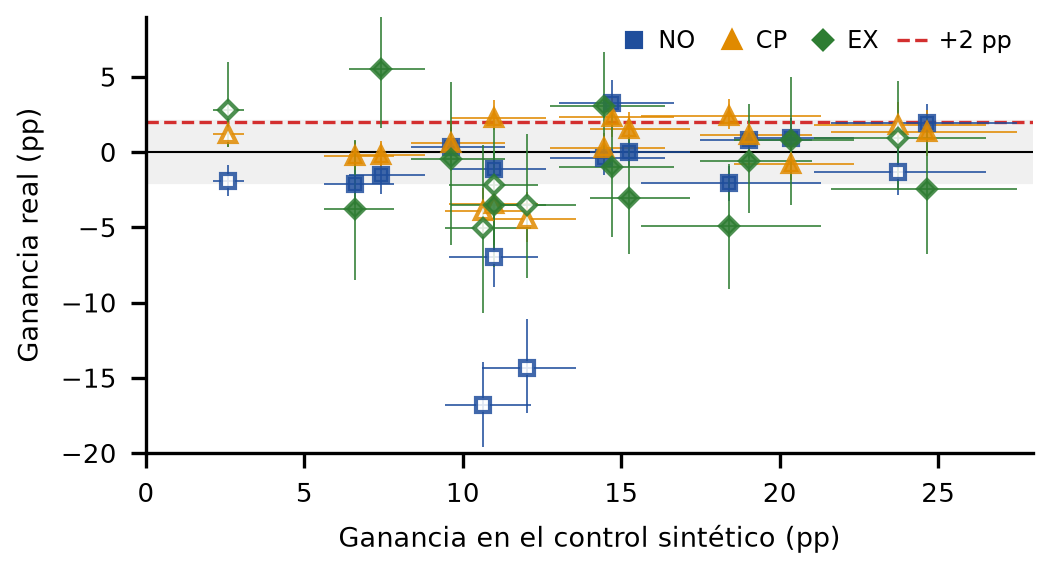
\includegraphics[width=0.7\textwidth]{fig_dispersion_es.png}
\caption{Ganancia en el control sintético frente a la ganancia en cada fuente real, con IC del 95\,\% por imágenes (17 bloques H3--H17; rellenos: exposición igual; vacíos: desigual o temprana; H3 queda fuera de escala). Banda gris: $\pm2$ pp. $\rho$ de Spearman con IC \emph{bootstrap} de bloques: NO +0,37 [$-$0,11; +0,75], CP +0,24 [$-$0,21; +0,62], EX $-0{,}05$ [$-$0,55; +0,51]; con exposición igual (11), NO +0,63 [0,00; +1,00]. Estaba en el cuerpo del artículo hasta la revisión del 27/10.}
\end{figure}

\section{Búsqueda bibliográfica}
Tres búsquedas en Scopus exportadas el 13/10/2026: ecuación principal (A y B, más al menos uno de C, D o E; 155 registros), dos ecuaciones complementarias (8) y oclusión sintética frente a real sin limitarse a personas (71). De ellas salieron los cinco artículos semilla (PRNet++, WALT, MLFFCSP, CamPed y el YOLOX con transferencia de dominio); la búsqueda se apoyó en Scopus AI y en Claude, y la selección la hicieron los autores leyendo los artículos. Cadenas exactas, copiadas del historial de búsquedas de Scopus:

\noindent\textbf{Ecuación principal (155 registros)}\\
{\ttfamily\footnotesize\raggedright TITLE-ABS-KEY ( ( ( pedestrian* or person or persons or people or human or humans ) W/4 detect* ) AND ( occlu* OR "partially visible" OR "partial visibility" OR "crowded scene" ) AND ( ( occlu* W/5 ( augment* or synthetic* or simulat* or artificial* or generat* or inpaint* or diffusion or paste or pasted or pasting or erasing ) ) OR "random erasing" OR cutout OR "copy paste" OR "low light" OR "low illumination" OR "poor illumination" OR "poor lighting" OR "dim light" OR "dark scene" OR "dark environment" OR "dark image" OR darkness OR night* OR nocturnal OR exdark OR nightowls OR "cross-dataset" OR "cross-domain" OR "domain gap" OR "domain shift" OR "dataset bias" OR "domain generali{?}ation" OR "out-of-distribution" OR "sim-to-real" OR "synthetic-to-real" OR "real occlusion" OR "natural occlusion" OR "real-world occlusion" OR ( generali{?}ation W/5 ( dataset* or domain* ) ) ) ) AND PUBYEAR > 2021 AND PUBYEAR < 2027 AND ( DOCTYPE ( ar ) OR DOCTYPE ( cp ) OR DOCTYPE ( re ) ) AND LANGUAGE ( english ) AND ( subjarea ( COMP ) OR subjarea ( ENGI ) ) AND NOT TITLE ( thermal OR infrared OR multispectral OR lidar OR radar OR "point cloud" )\par}

\noindent\textbf{Ecuación complementaria (8 registros)}\\
{\ttfamily\footnotesize\raggedright TITLE-ABS-KEY ( ( ( pedestrian* or person or persons or people or human or humans ) W/4 detect* ) AND ( ( occlu* W/5 ( augment* or synthetic* or simulat* or artificial* or generat* or inpaint* or diffusion or paste or pasted or pasting or erasing ) ) OR "random erasing" OR cutout OR "copy paste" ) AND ( "low light" OR "low illumination" OR "poor illumination" OR night* OR nocturnal OR exdark OR nightowls OR "cross-dataset" OR "cross-domain" OR "domain gap" OR "domain shift" OR "real occlusion" OR "natural occlusion" OR "real-world occlusion" ) ) AND ( DOCTYPE ( ar ) OR DOCTYPE ( cp ) OR DOCTYPE ( re ) ) AND LANGUAGE ( english )\par}

\noindent\textbf{Oclusión sintética frente a real (71 registros)}\\
{\ttfamily\footnotesize\raggedright TITLE-ABS-KEY ( ( occlu* W/5 ( synthetic* or simulat* or artificial* ) ) AND ( "real occlusion" OR "natural occlusion" OR "real-world occlusion" OR "naturally occluded" OR "real occluded" ) ) AND ( DOCTYPE ( ar ) OR DOCTYPE ( cp ) OR DOCTYPE ( re ) ) AND LANGUAGE ( english )\par}

\noindent  Después de dos revisiones (20/10/2026) se añadieron, por búsqueda dirigida y tras leer su resumen o su texto, Taori et al. (2020), Pytel et al. (2021), Kortylewski et al. (2020), Wang et al. (2020), Ghiasi et al. (2021) y Geirhos et al. (2020). Todas las referencias se verificaron en Crossref o arXiv.

\section{Licencias, datos y cumplimiento}
\noindent\textbf{Licencias.} ExDark: imágenes bajo sus términos de uso para investigación académica no comercial (\url{https://github.com/cs-chan/Exclusively-Dark-Image-Dataset}). CityPersons (imágenes de Cityscapes): uso no comercial, citar el conjunto, sin redistribuir (\url{https://www.cityscapes-dataset.com/license/}). NightOwls: uso no comercial, citar el conjunto, sin redistribuir; se permiten derivados abstractos como modelos entrenados (\url{https://www.nightowls-dataset.org}). El proyecto no redistribuye imágenes; publica identificadores, anotaciones derivadas, códigos y pesos.

\noindent\textbf{Material del repositorio.} \path{PREREGISTRO_*.md}, \path{CAMBIOS_PROTOCOLO.md} y \path{protocolo_congelado.json} (hipótesis y huellas); \path{informes/analisis_final/registro_corridas.csv} (corridas); \path{celdas_completas.csv}, \path{bootstrap*.csv}, \path{miss_rate*.csv} y \path{revision_sp.json} (cifras e intervalos); \path{config/} y \path{argos_lib/} (aumento y control); \path{16_oclusion_proxy.py} y \path{gt_test_proxy.json} (indicador de ExDark); \path{17_fiabilidad_anotacion.py} (estudio de $\kappa$, sin nombres de anotadores); \path{31_realismo.py} (H13).

\begin{table}[H]\centering\small
\caption{Lista REFORMS (Kapoor et al., 2024) resumida: dónde se atiende cada bloque.}
\begin{tabular}{@{}p{5.2cm}p{11cm}@{}}\toprule
Bloque & Dónde \\\midrule
Objetivos y afirmaciones & Introducción; tabla~I del artículo; tabla~\ref{tab:s-hip} \\
Reproducibilidad computacional & Repositorio público \url{https://github.com/jhanrq8888/argos-occlusion-transfer}; pesos con DOI en Zenodo al publicarse; versiones en la sección 3 \\
Datos y preprocesamiento & Sección Datos del artículo; tabla de aumento y control; licencias \\
Separación entrenamiento--prueba & Control con imágenes y oclusores no vistos; validación nunca ocluida salvo \texttt{val\_ocluido} para seleccionar \\
Selección de modelos & Tabla~\ref{tab:s-registro} (época evaluada de cada corrida); bloques de exposición fija como evidencia primaria \\
Métricas e incertidumbre & Tablas~\ref{tab:s-celdas} y~\ref{tab:s-estad}; MR$^{-2}$ en la tabla~\ref{tab:s-extra}; AP@0.5:0.95 en \path{informes/analisis_final/ap_estricto.csv} (ninguna de las 21 celdas de los siete primeros bloques supera el umbral) \\
Generalización y limitaciones & Discusión del artículo (tres categorías) \\
\bottomrule\end{tabular}\end{table}

\noindent\textbf{Guía práctica.} (1) Un banco de oclusión sintética sirve como control positivo de que un aumento está bien implementado, no como prueba de robustez. (2) Para afirmar robustez a la oclusión hace falta un conjunto de oclusión real anotada del dominio de uso, aunque sea pequeño, y comparar con la misma exposición al entrenamiento. (3) En una comparación descriptiva, no controlada, entrenar con datos anotados del dominio dio mucho más que cualquier aumento (0,59 frente a 0,24 en CityPersons \emph{heavy}); compararlo con el mismo presupuesto queda pendiente. (4) Reportar siempre la época de los pesos de V1 y V3.

\end{document}
